\styledchapter[Orkestratietools om platformen te beheren]{orkestratietools-om-platformen-te-beheren}
Om resources in een cloud platform te beheren kan gebruik gemaakt worden van een portaal. In een portaal kunnen databases, servers en netwerken aangemaakt worden om een infrastructuur te creëren. Omdat een portaal uitgebreid en complex kan zijn, moet de developer een infrastructuur kunnen opzetten zonder het gebruik van een portaal. Dit is mogelijk met \acrfull{iac} orkestratietools. \Acrshort{iac} zal als eerst worden uitgelegd. Vervolgens worden verschillende \Acrshort{iac} orkestratietools met elkaar vergeleken. Als laatst wordt een experiment uitgevoerd om de haalbaarheid met een orkestratietool te valideren.

\section{Wat is infrastructure as code?}\label{subsec:ch5-wat-is-infrastructure-as-code}
\acrshort{iac} is een manier om een infrastructuur op te zetten binnen een cloud platform zonder gebruik te maken van een interface zoals een portaal. De gewenste infrastructuur wordt beschreven waarna de orkestratietool de gewenste situatie een realiteit probeert te maken \cite{iac-amazon-web-services-in-action}.

De manier waarmee een orkestratietool de infrastructuur aanmaakt, wijzigt of verwijderd is met een plan. In het plan staat welke resources moeten bestaan om aan de gewenste situatie te voldoen. Vaak gaat dit gepaard met configuratie zoals een naam, locatie of tags. In \autoref{fig:ch5-iac-plan-example} is een voorbeeld van een plan als een YAML-bestand te zien. YAML is een bestandstype dat vaak wordt gebruikt voor configuratie. Het plan beschrijf op welke cloud platform dit uitgevoerd moet worden (regel 12) en wat er aangemaakt moet worden. In dit geval is het een resource group (regel 16) met als configuratie een naam (\(myTFResourceGroup\)) en locatie (\(westus2\)).

\begin{figure}[hbt!]
  \centering
  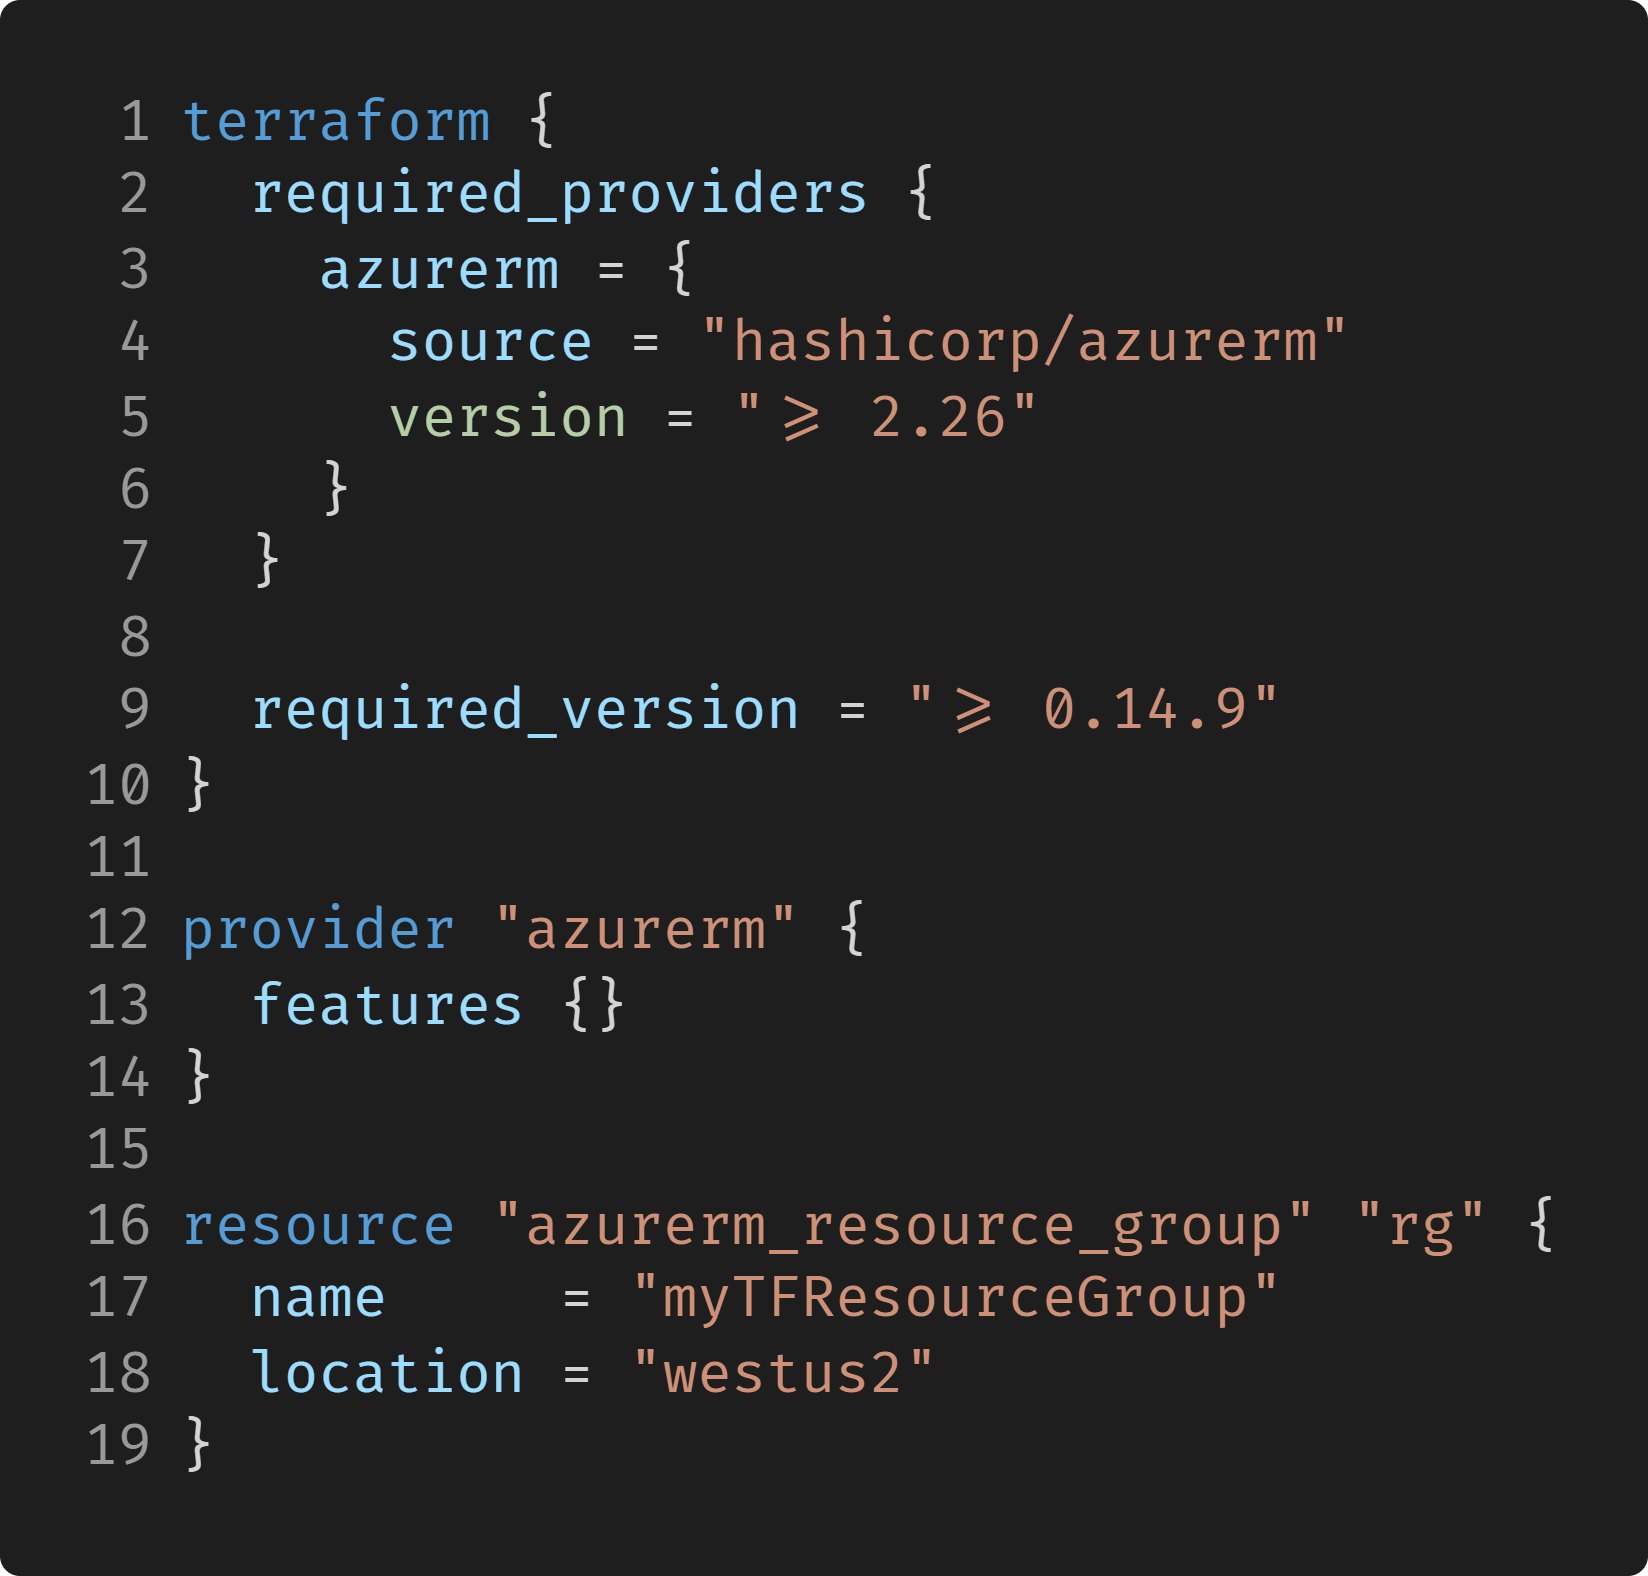
\includegraphics[width=0.5\textwidth]{chapter-5/iac-plan-example.png}
  \caption{Voorbeeld van een \acrfull{iac} plan \cite{terraform-plan-example}}
  \label{fig:ch5-iac-plan-example}
\end{figure}

Een \Acrshort{iac} volgt een proces om aan de gewenste situatie te voldoen. In \autoref{fig:ch5-iac-process} is te zien hoe zo een proces verloopt. Zodra de orkestratietool start, wordt zowel het plan als de situatie in de cloud platform gecontroleerd en met elkaar vergeleken. In stap 1 is het plan valide, maar de situatie in de cloud platform niet. Dit betekent bijvoorbeeld dat er in het plan staat dat er een resource group moet bestaan met een naam en locatie zoals het beschreven staat in \autoref{fig:ch5-iac-plan-example}, maar dit niet bestaat in de cloud platform. In de volgende stap wordt de resource aangemaakt door de \Acrshort{iac} om aan de gewenste situatie te voldoen. De wijzigingen gebeuren programmatisch en wordt gedaan door de \Acrshort{iac}. Er is geen tussenkomst van een persoon of interface nodig. 

\begin{figure}[hbt!]
  \centering
  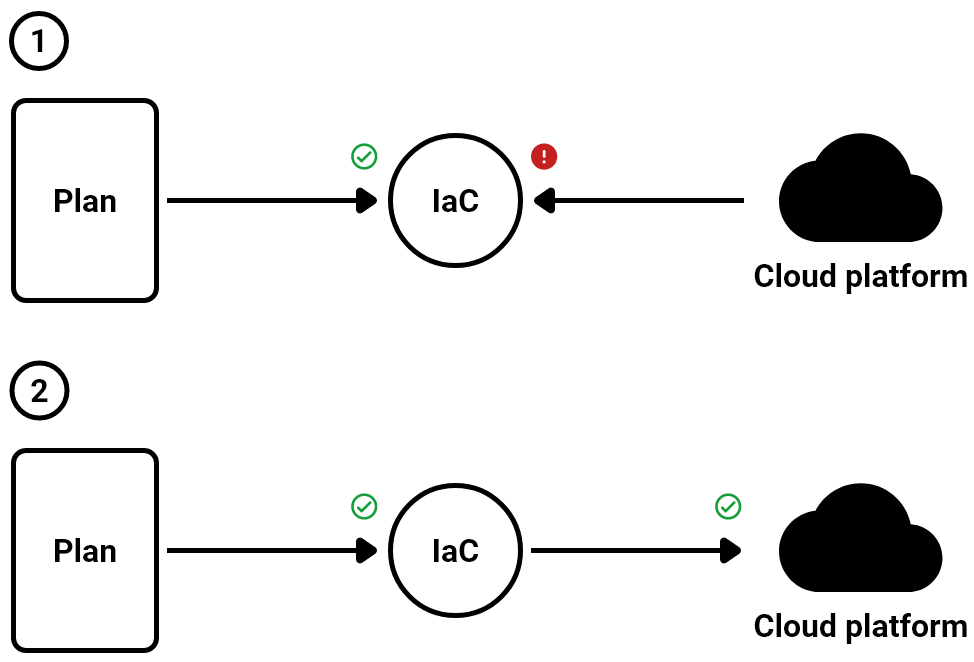
\includegraphics[width=0.75\textwidth]{chapter-5/iac-process.png}
  \caption{Proces van een \acrfull{iac} om aan de gewenste situatie te voldoen}
  \label{fig:ch5-iac-process}
\end{figure}

\section{Orkestratietools vergeleken met elkaar}\label{subsec:ch5-orkestratietools-vergeleken-met-elkaar}
Om een keuze te maken tussen \acrshort{iac} orkestratietools kunnen zogenoemde "knock-out"\space criteria opgesteld worden. Een \acrshort{iac} orkestratietool valt af zodra de tool niet voldoet aan één van de criteria. In \autoref{table:knock-out-criteria-orchestration-tools-that-manage-cloud-computing-platformen} zijn de knock-out criteria te vinden. De criteria zijn samenwerking met NGTI opgesteld. 

\begin{table}[hbt!]
  \centering
  \caption{Knock-out criteria voor orkestratietools dat cloud computing platformen beheert}
  \vspace*{.5\baselineskip}
  \begin{tabular}{|p{.2\linewidth}|p{.69\linewidth}|}
  \hline
  \textbf{Criteria} & \textbf{Toelichting} \\ \hline
    Programmatisch beheren
    &
    Het orkestratietool moet via code een resources kunnen aanmaken, wijzigen en verwijderen. 
    \\ \hline

    Ondersteuning voor cloud \newline computing \newline platformen
    &
    Om platform-agnostisch te zijn moet de orkestratietool minstens twee cloud computing platformen ondersteunen waarop een ML model getraind kan worden.
    \\ \hline

    Uitgebreide \newline documentatie
    &
    De documentatie moet toegankelijk en duidelijk zijn. Ook moet de documentatie moet tutorials, concepten en een reference bevatten.
    \\ \hline
  \end{tabular}
  \label{table:knock-out-criteria-orchestration-tools-that-manage-cloud-computing-platformen}
\end{table}

\newpage

Voor de keuzes uit de tools is onderzoek gedaan op het internet en een enquête geraadpleegd van Stack Overflow \cite{stack-overflow-survey-2020}. De enquête is ingevuld door developers en bevat vragen over de ervaring met frameworks, technologieën en de website zelf. Uit de vraag over welke frameworks, libraries en tools het meest gebruikt werkt, kwam Ansible, Terraform, Puppet en Chef naar boven \cite{stack-overflow-survey-2020-popular-framework-libraries-tools}. Volgens een vraag over de meest geliefd en gevreesde frameworks, libraries en tools zijn Ansible en Terraform het meest geliefd en Puppet en Chef het meest gevreesd \cite{stack-overflow-survey-2020-loved-dreaded-framework-libraries-tools}. Uit algemeen onderzoek naar orkestratietools is, naast de bovengenoemde tools, Pulumi naar voren gekomen als kandidaat \cite{pulumi}. Ansible, Terraform en Pulumi zijn in \autoref{table:orchestration-tools-compared-against-knock-out-criteria} tegen de knock-out criteria gehouden.

\begin{table}[hbt!]
  \centering
  \caption{Knock-out criteria tegen orkestratietools dat cloud computing platformen beheerd}
  \vspace*{.5\baselineskip}
  \begin{tabular}{|p{.15\linewidth}|p{.245\linewidth}|p{.245\linewidth}|p{.245\linewidth}|}
  \hline
  \textbf{Orkestratie-\newline tools} & \textbf{Programmatisch \newline beheren} & \textbf{Ondersteuning voor cloud computing \newline platformen} & \textbf{Uitgebreide \newline documentatie} \\ \hline
    \textbf{Ansible} &
    Nee, orkestratie gaat via een YAML-bestand \cite{ansible-code} &
    AWS, Google Cloud en Azure. 11 platformen in totaal \cite{ansible-cloud-platforms} &
    Uitgebreide documentatie met tutorials, references en migration guide \cite{ansible-docs}
    \\ \hline

    \textbf{Pulumi} &
    Ja, orkestratie via CLI of TypeScript, JavaScript, Python, .NET en Go \cite{pulumi-code} &
    AWS, Google Cloud en Azure. 13 platformen in totaal \cite{pulumi-cloud-platforms} &
    Uitgebreide documentatie met tutorials en references \cite{pulumi-docs}
    \\ \hline

    \textbf{Terraform} &
    Nee, orkestratie gaat via een YAML-bestand \cite{terraform-code} &
    AWS, Google Cloud en Azure. 5 platformen in totaal \cite{terraform-cloud-platforms} &
    Uitgebreide documentatie met tutorials, references en video's \cite{terraform-docs}
    \\ \hline
  \end{tabular}
  \label{table:orchestration-tools-compared-against-knock-out-criteria}
\end{table}

In \autoref{table:orchestration-tools-compared-against-knock-out-criteria} is te zien dat de drie orkestratietools gelijk zijn als het gaat om de ondersteuning van cloud platform en documentatie. Programmatisch beheren kan met Ansible en Terraform alleen door middel van een YAML-bestand in tegenstelling tot Pulumi dat via code een plan kan uitvoeren. Omdat het praktischer voor de PoC is om via code een plan uit te voeren, is er voor gekozen om met Pulumi verder te werken. In het volgende hoofdstuk zal een experiment met Pulumi uitgevoerd worden om te valideren of Pulumi geschikt is.

\section{Experiment met de orkestratietool Pulumi}\label{subsec:ch5-experiment-met-de-orkestratietool-pulumi}
Het idee achter het experiment is om te achterhalen of Pulumi een geschikte orkestratietool is. Op dit moment in het afstudeerproces wordt er verwacht dat de PoC een front-end krijgt dat praat door middel van een \acrfull{rest} \Acrshort{api} met een back-end. De back-end zal vervolgens gebruik maken van de orkestratietool om te praten met een cloud platform. Om de PoC na te bootsen op kleinere schaal wordt er bij het experiment gebruik gemaakt van een client waarbij een opdracht met behulp van een \Acrshort{rest} \Acrshort{api} naar een Node.js server wordt verstuurd. De Node.js server stuurt om zijn beurt opdrachten naar Pulumi die communiceert met Google Cloud. Voor het experiment is arbitrair gekozen voor het cloud platform; de PoC moet ten slotte platform-agnostisch zijn.

Het experiment is als sequence diagram uitgewerkt in \autoref{fig:sd-pulumi-experiment}. Hierin is goed te zien welke acties gedaan worden en door welke actor. In de sequence diagram is ook te zien wat voor taak wordt uitgevoerd aan de hand van de naam tussen de actoren.

\begin{figure}[hbt!]
  \centering
  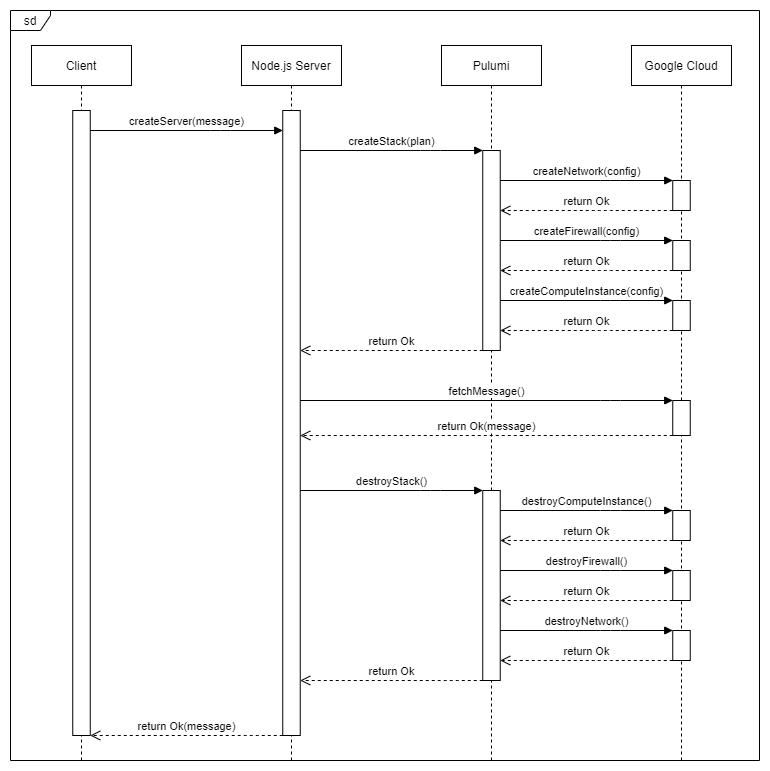
\includegraphics[width=.99\textwidth]{chapter-5/sd-pulumi-experiment.png}
  \caption{Sequence diagram van het experiment met orkestratietool Pulumi}
  \label{fig:sd-pulumi-experiment}
\end{figure}

\newpage

De Node.js server is vrij simpel en bevat één endpoint op regel 12 genaamd /api/run-python-code (\autoref{fig:pulumi-experiment-nodejs-base}). In deze \(POST\) endpoint wordt een stack aangemaakt, een \(GET\) request uitgevoerd naar de aangemaakte compute instance en vervolgens wordt de stack weer verwijderd. Een stack is de manier hoe Pulumi een plan beschrijft.

\begin{figure}[hbt!]
  \centering
  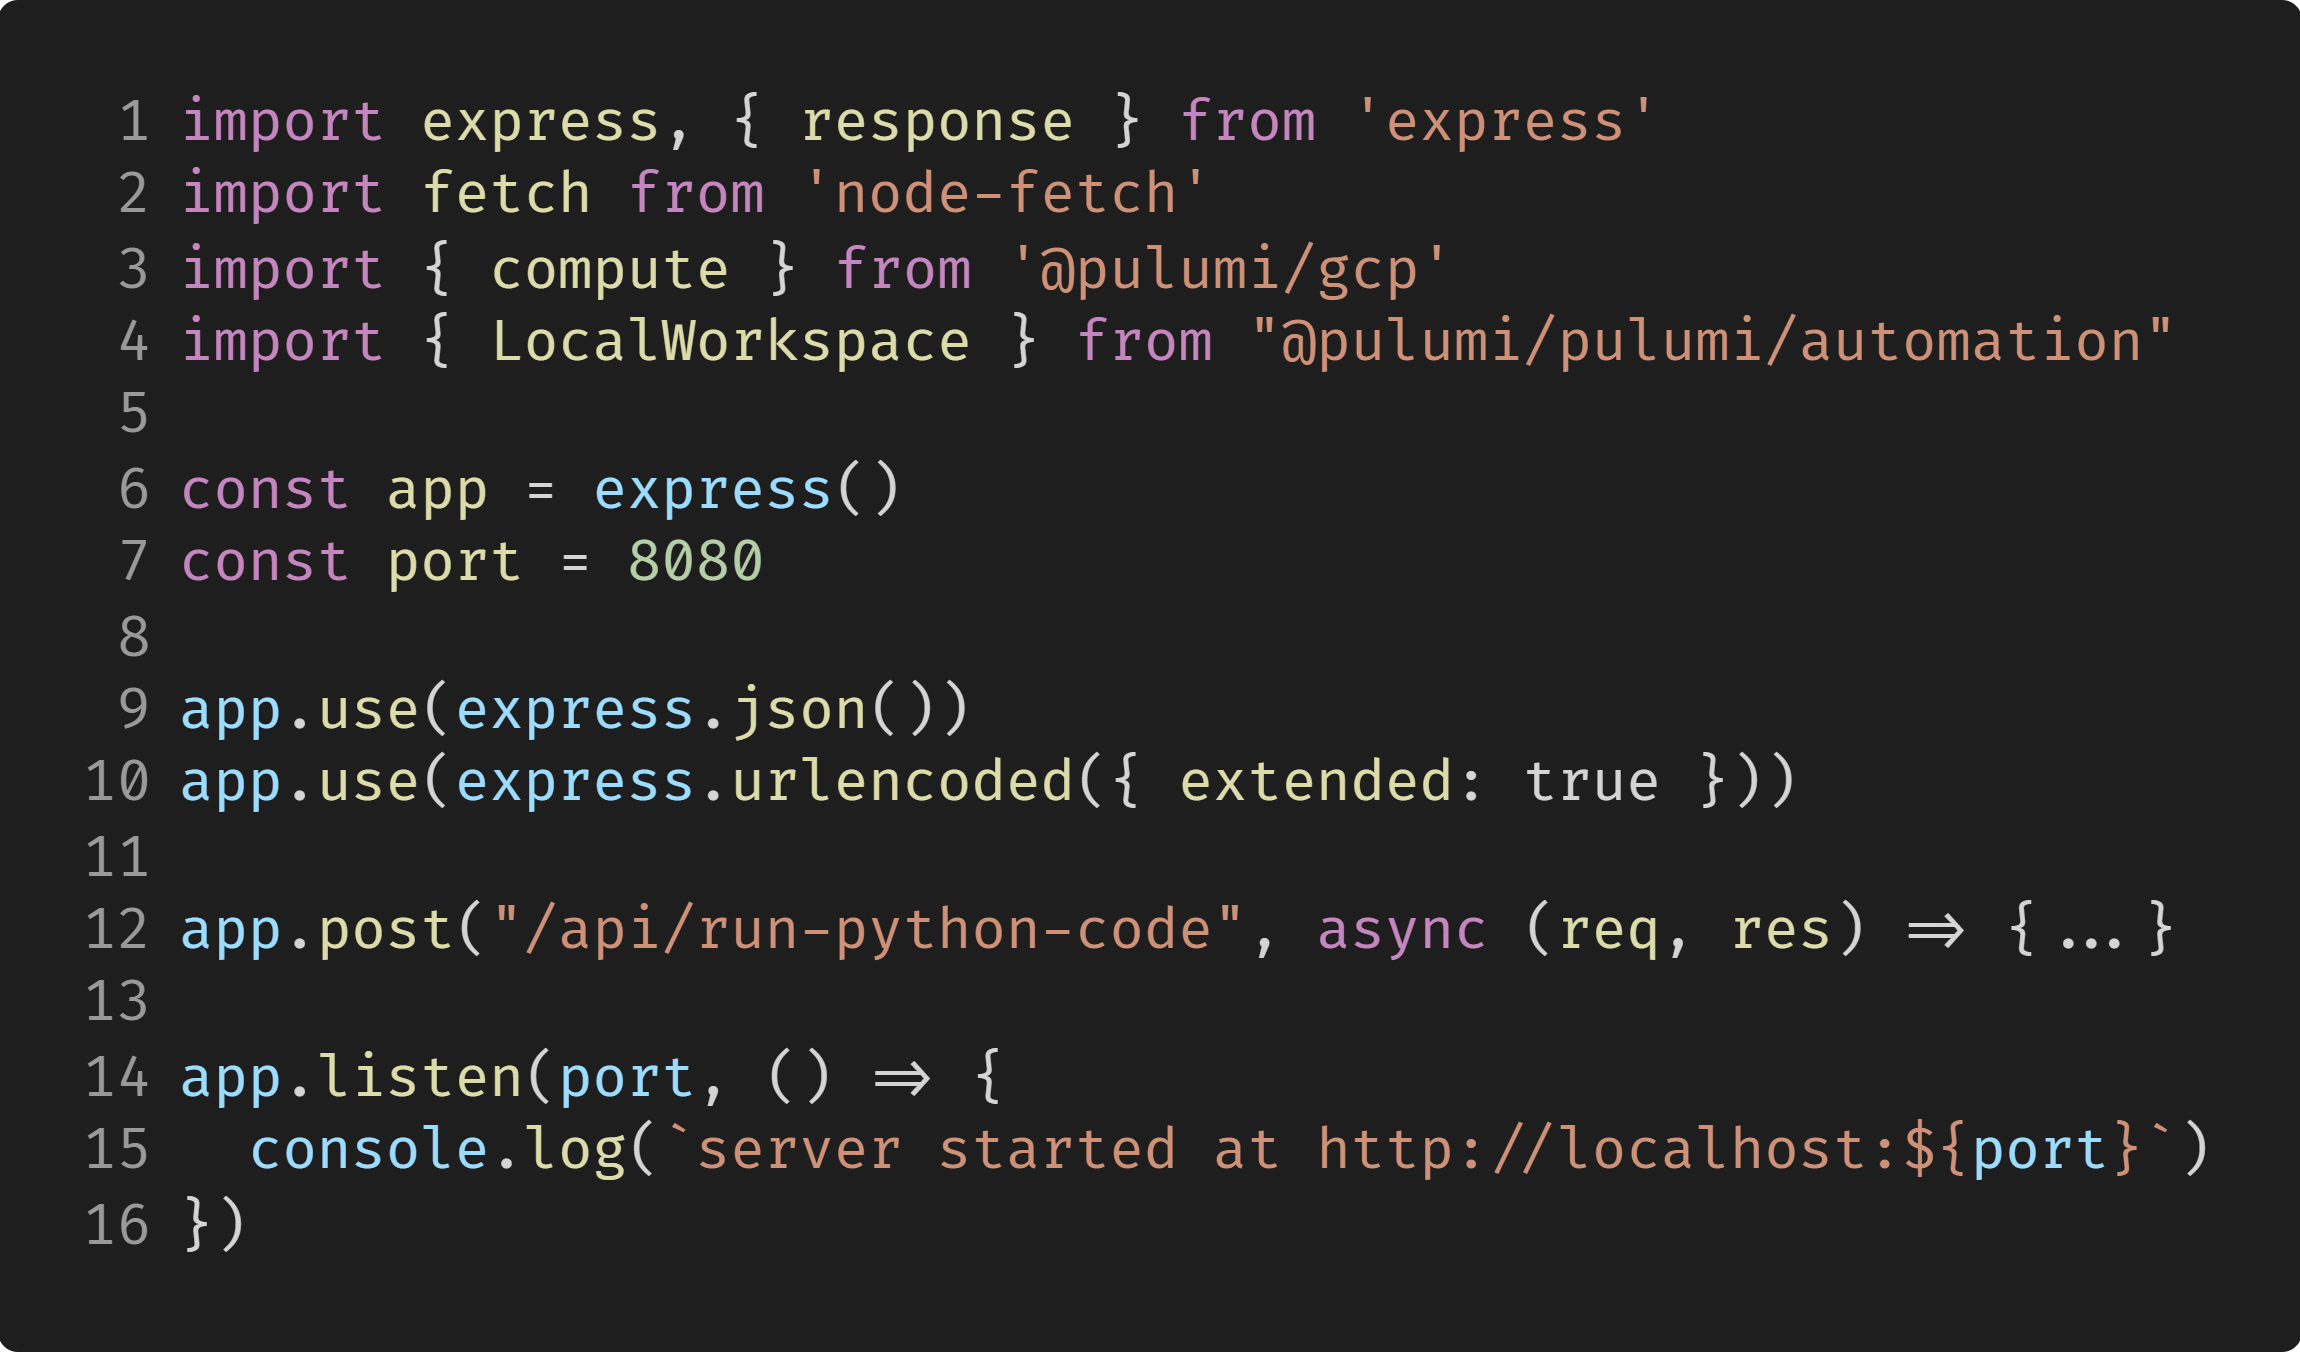
\includegraphics[width=.75\textwidth]{chapter-5/pulumi-experiment-nodejs-base.png}
  \caption{Node.js server voor het experiment met orkestratietool Pulumi}
  \label{fig:pulumi-experiment-nodejs-base}
\end{figure}

In de stack worden drie resources aangemaakt: een network, een firewall en een compute instance (\autoref{fig:pulumi-experiment-plan-simple}). De compute instance moet een HMTL bestand serveren met een bericht dat de client heeft gespecificeerd. 

\begin{figure}[hbt!]
  \centering
  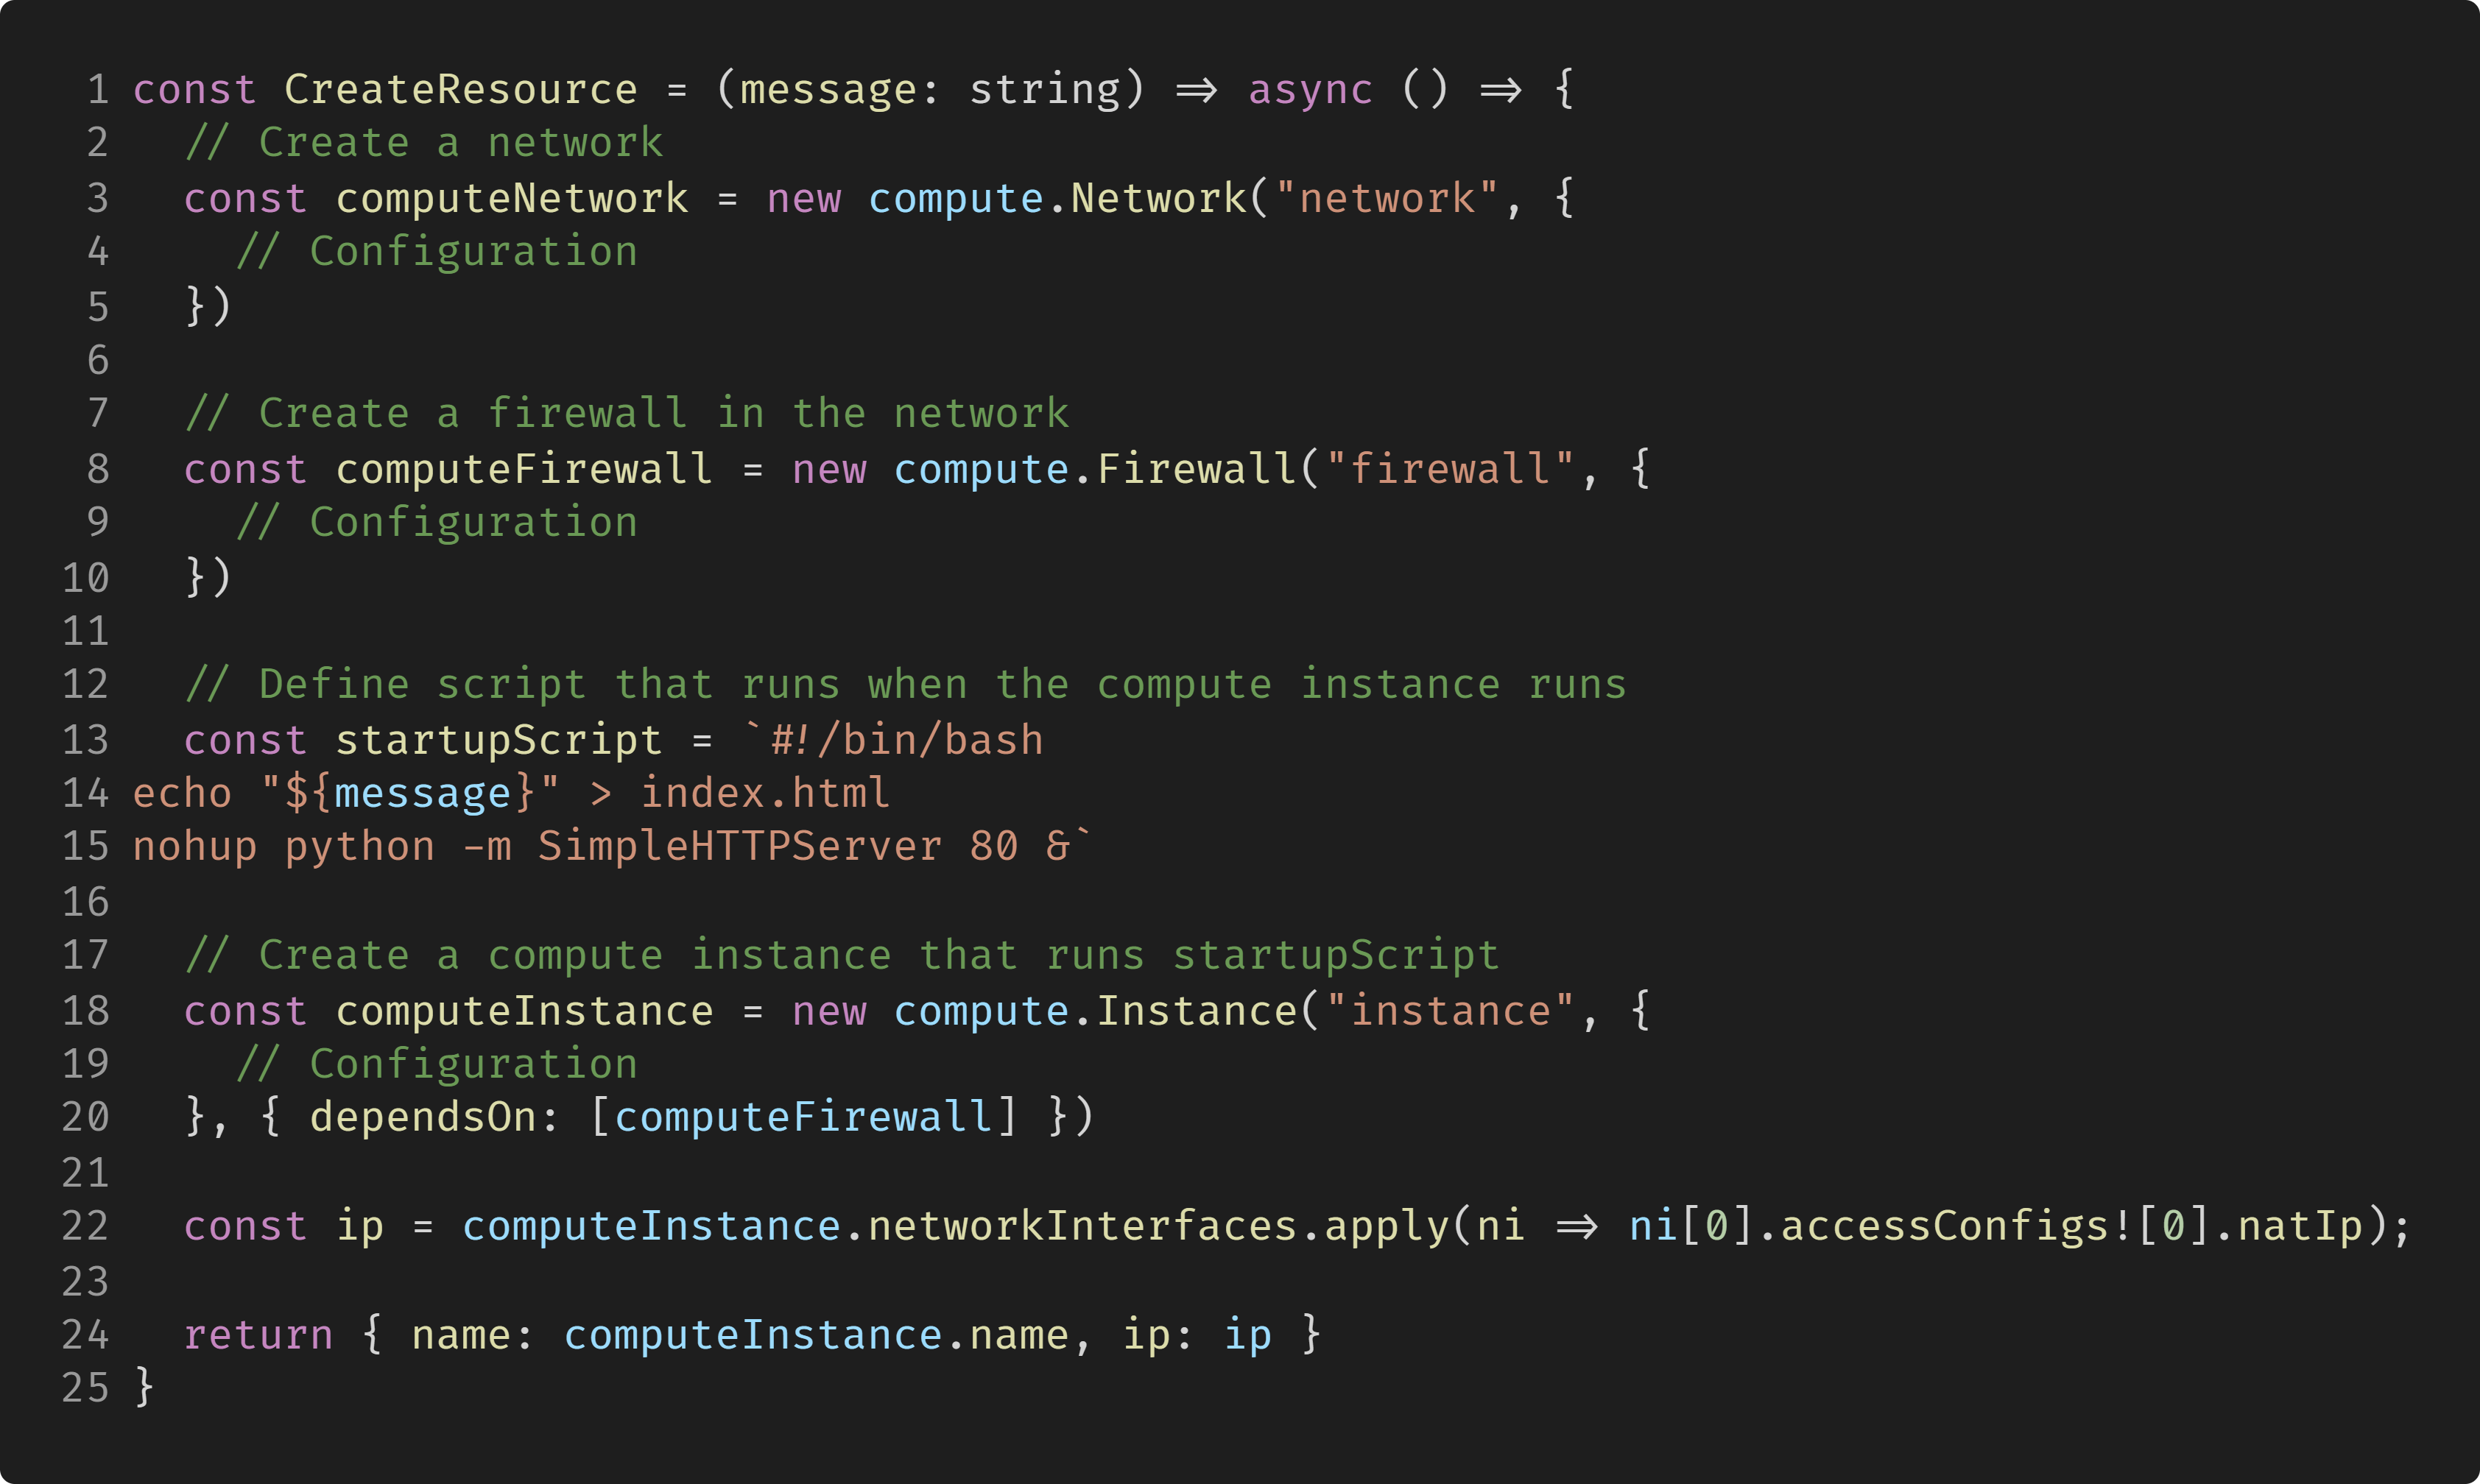
\includegraphics[width=.8\textwidth]{chapter-5/pulumi-experiment-plan-simple.png}
  \caption{De stack voor het experiment}
  \label{fig:pulumi-experiment-plan-simple}
\end{figure}

Elke resource heeft zijn eigen configuratie om te te zorgen dat het HTML bestand beschikbaar is voor de buitenwereld. De code met de volledige configuratie is te vinden in bijlage \ref{appendix:stack-configuration-from-experiment-with-pulumi}.

In \autoref{fig:pulumi-experiment-endpoint} is te zien wat er in de POST endpoint gebeurt. Als eerst wordt een stack in geheugen aangemaakt met behulp van de code in \autoref{fig:pulumi-experiment-plan-simple}. Na het aanmaken wordt de stack uitgevoerd met de \(stack.up()\) functie op regel 12. Nadat de stack is aangemaakt in Google Cloud wordt een \(GET\) request uitgevoerd naar de server op regel 15. Nadat de request voltooid is wordt de stack verwijderd uit Google Cloud (regel 21) met \(stack.destroy()\) en wordt het bericht teruggestuurd naar de client.

\begin{figure}[hbt!]
  \centering
  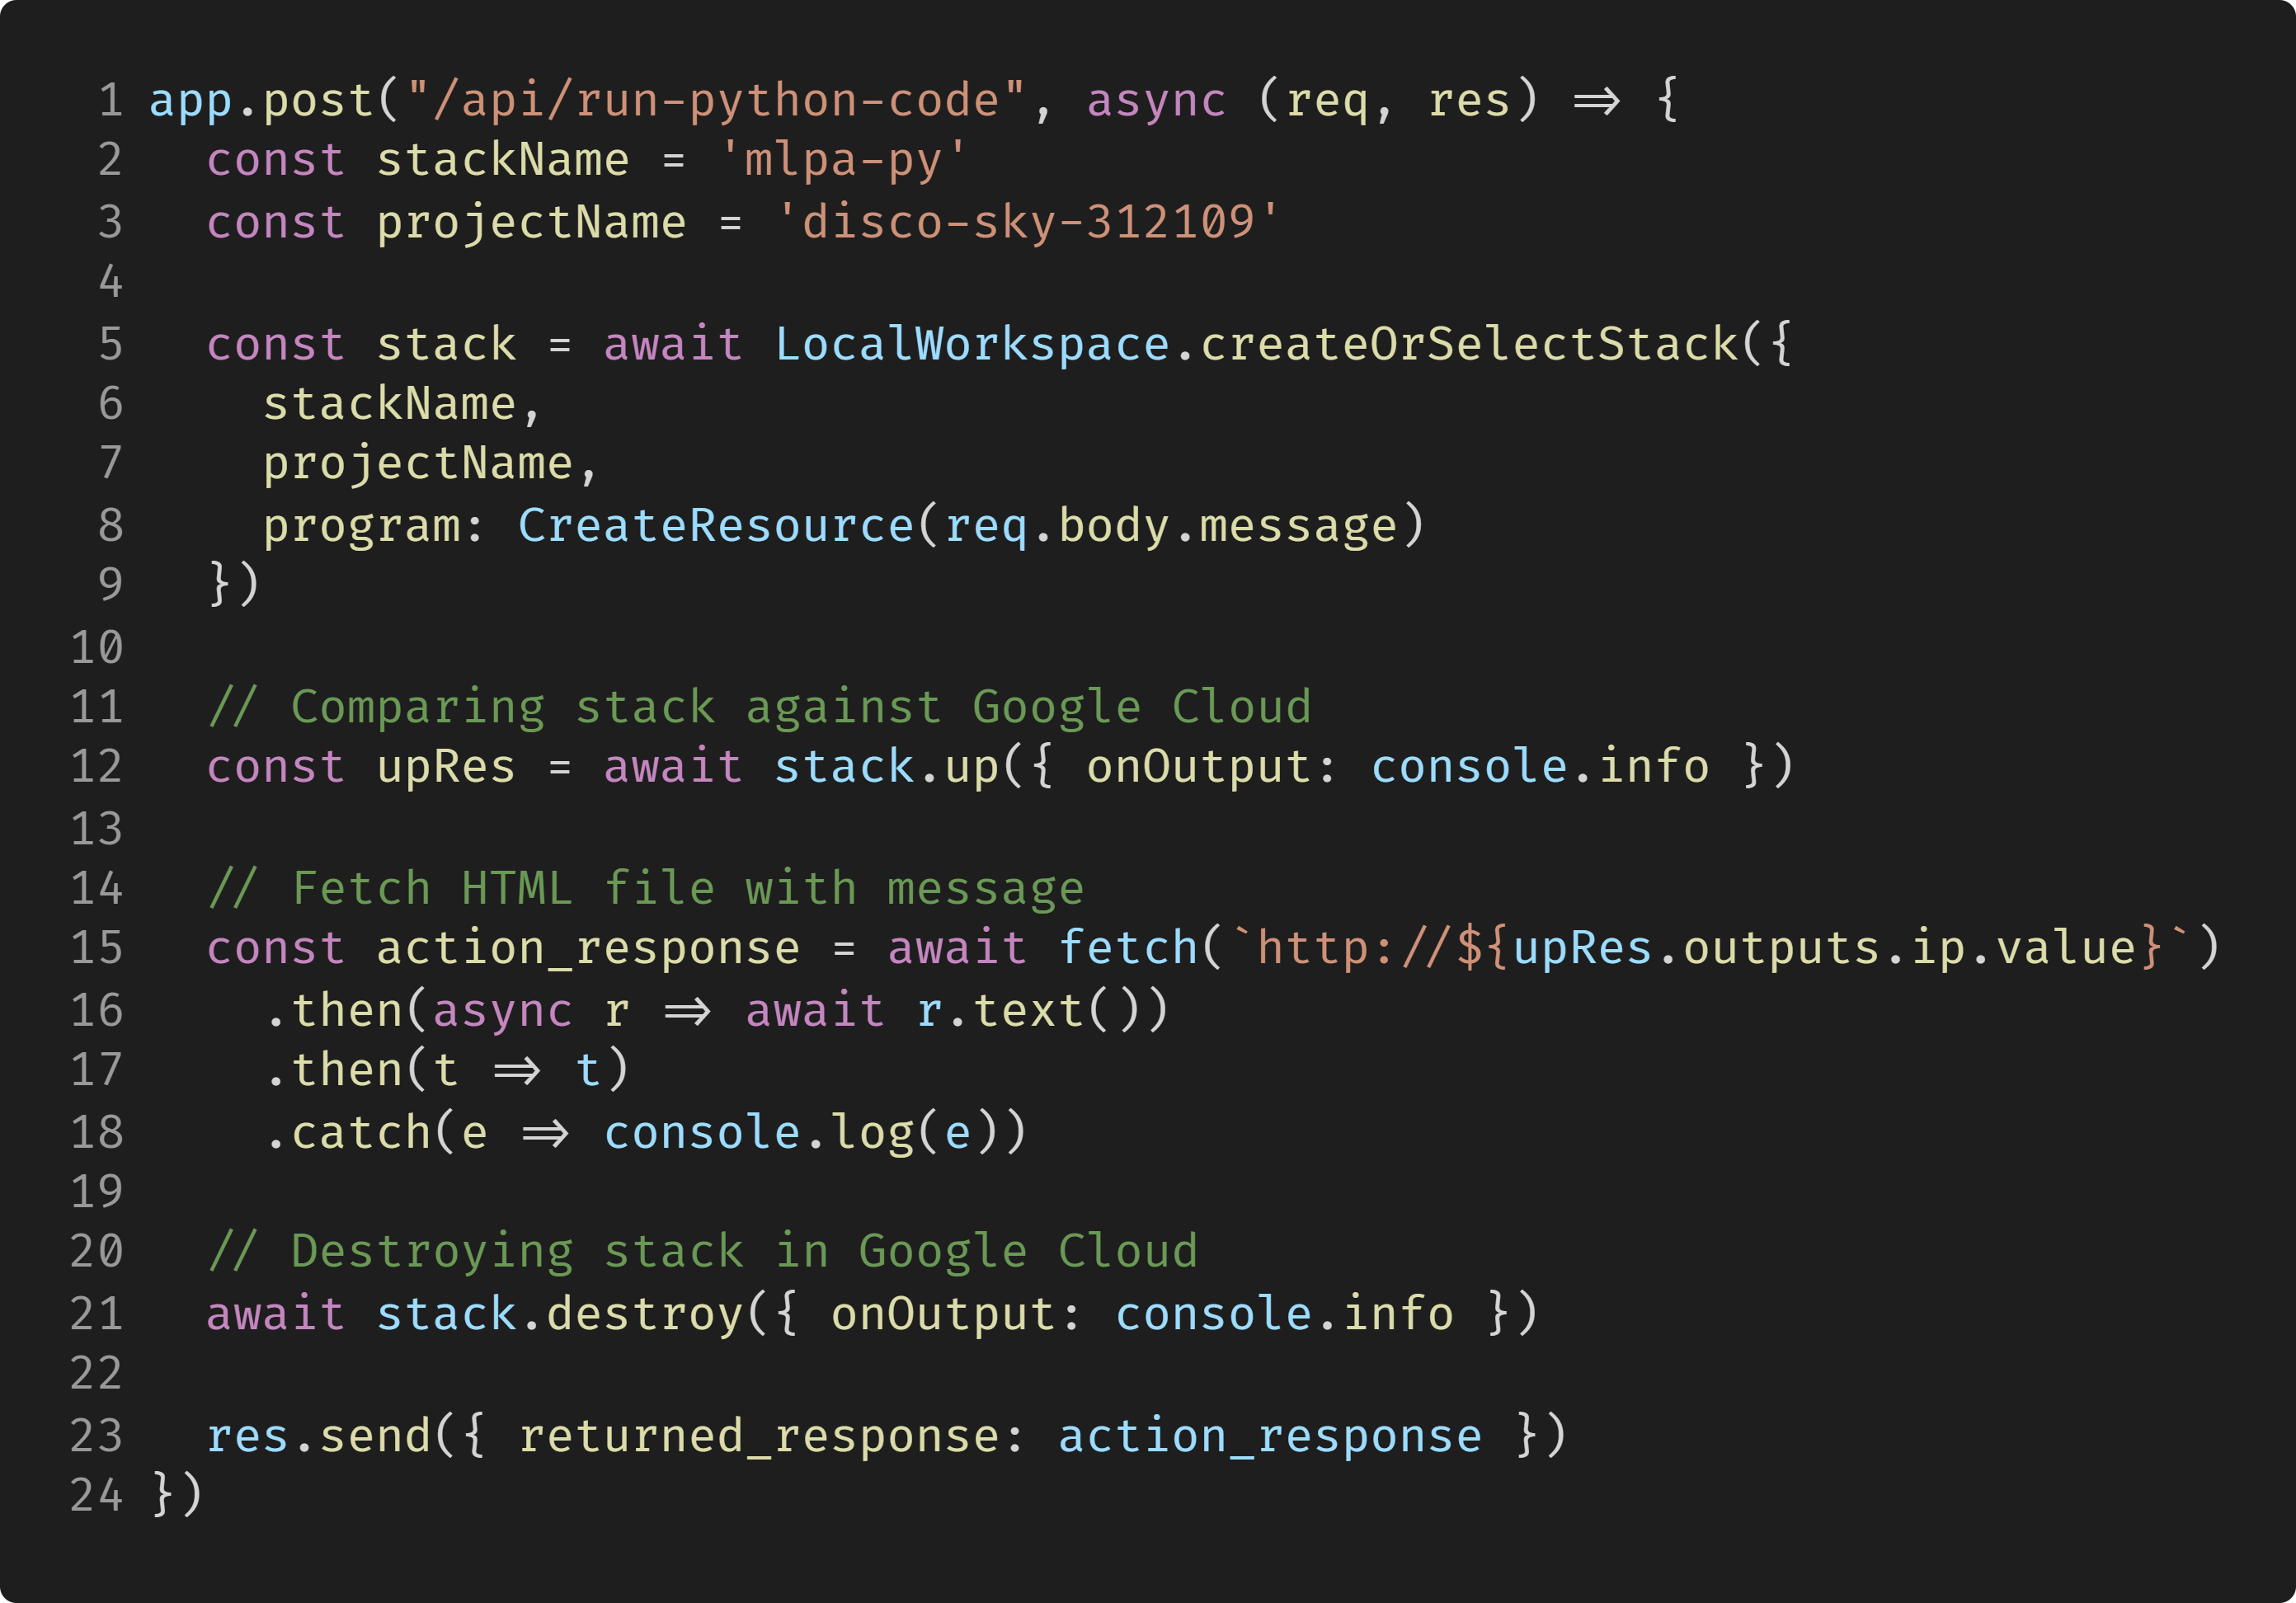
\includegraphics[width=.8\textwidth]{chapter-5/pulumi-experiment-endpoint.png}
  \caption{POST endpoint van de Pulumi experiment}
  \label{fig:pulumi-experiment-endpoint}
\end{figure}

\section{Conclusie}\label{subsec:ch5-conclusie}
In dit hoofdstuk is er onderzoek gedaan naar het antwoord op de deelvraag: \textbf{D2: Hoe kan een orkestratietool verschillende cloud computing platformen beheren om een machine learning pipeline op te zetten?} Het onderzoek is uitgevoerd met behulp van digitale bronnen en een experiment.

Een orkestratietool is een manier om resources aan te maken, aan te passen en te verwijderen. De tool doet dit zonder het gebruik van een online portaal of interventie van een developer. Het managen van resources wordt gedaan op basis van een plan en de huidige situatie binnen de cloud platform. In het plan staat welke resources moeten bestaan en met welke configuratie. Het plan kan beschreven worden in een YAML-bestand of door middel van code. De orkestratietool vergelijkt vervolgens het plan met de huidige situatie en zorgt er voor dat de situatie voldoet aan het plan.

De orkestratietool Pulumi is een valide optie uitgaand van het experiment. Pulumi heeft uitstekende documentatie en laat middels output zien wat er gebeurd als Pulumi wordt uitgevoerd. Ook is de manier waarop Pulumi werkt (\autoref{fig:pulumi-experiment-plan-simple}) simpel en makkelijk te volgen.